Para este ejercicio se implemento el decodificador de direcciones con un integrado 74LS138 y lógica combinacional.
Valiendonos de que únicamente se utilizaran 4 periféricos, es posible asignar cantidades de memoria por demás a los mismos.
Quedando de la siguiente manera la tabla de direcciones.
\begin{table}[H]
\centering
\begin{tabular}{cccc}
\hline
\textbf{Adress} & \textbf{Dispositivo} & \textbf{Binario} \textbf{Comienzo} & \textbf{Binario Fin} \\ \hline
C000 & ROM16K & 1100000000000000 & 1111111111111111 \\
A800 & Entrada 8 Bits & 1010100000000000 & 1011111111111111 \\ 
A000 & Salida 8 Bits & 1010000000000000 & 1010011111111111 \\ 
2000 & RAM4K & 0010000000000000 & 0010111111111111 \\ \hline
\end{tabular}
\caption{Tabla de dispositivos y direcciones.}
\end{table}
Basta con conectar los siguientes bits con el decoder
\begin{align}
a_{14} \implies C\\
a_{15} \implies B\\
a_{11} \implies A
\end{align}
así también conectar las salidas $Y_0$ $Y_1$  con una compuerta or, al igual que las $Y_6$ $Y_7$ con otra.
quedando definidos los chip select de la siguiente manera.

\begin{figure}[H]
  \centering
  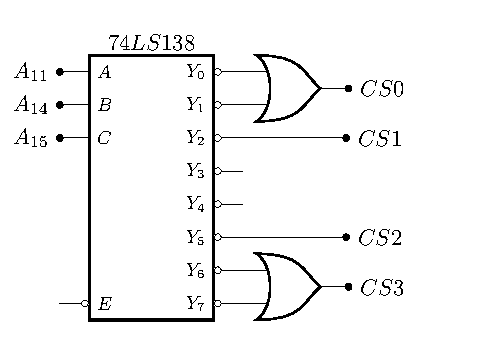
\includegraphics[width=.6\textwidth, page = 1]{ImagenesEjercicio2/Circuits.pdf}
  \caption{Diagrama en bloques}.
  \label{fig:fotofea}
\end{figure}